\documentclass{article}
\usepackage{amsmath,amsthm,amssymb}
\usepackage{mathtext}
\usepackage[T2A]{fontenc}
\usepackage[utf8]{inputenc}
\usepackage[english]{babel}
\usepackage{graphicx}
\usepackage{hyperref}
\usepackage{booktabs}
\usepackage{multirow}


\title{Mind Map Generation Using Large Language Models}
\author{Fedor Sobolevsky}
\date{May 2026}



\begin{document}
\maketitle
\begin{abstract}
    This project tackles the task of sentence-based mind map generation. The existing state-of-the-art methods for this task are graph-based, however, the great potential of approaches utilizing large language models (LLMs) is understudied. With careful prompt engineering and data processing, this study manages to achieve state-of-the-art performance on a mind map generation benchmark. The code for this project is available at: \url{https://github.com/TeoSable/llm-mind-maps}.
\end{abstract}



\section{Introduction}
Mind maps are a powerful tool for text comprehension and structuring, offering a convenient representation of information organized from key points to details. However, the process of manual mind map creation is generally time-consuming, limiting the usage of mind maps by the general public. One possible solution to this problem is automatic mind map generation, which enables effective information acquisition using mind maps without the cost of their manual creation.

Most studies in the field of automatic mind map generation focus on concept-based mind maps, i.\,e. mind maps containing key snippets from the source documents. However, it can be useful to generate a mind map that can be read like coherent text, making it an accessible way of hierarchical knowledge acquisition. This study will focus on this type of mind maps.

Recent approaches for automatic sentence-based mind map generation generally rely on graph-based methods and had been shown to achieve better performance than large language models (LLMs) at the time. However, with the rapid development of new and improved LLMs, such models become increasingly versatile tools for natural language processing (NLP) tasks. This raises the following question: can we achieve performance superior to previous graph-based methods using state-of-the-art large language models? This study provides a definitive answer to that question, showing that LLMs can in fact be effectively used for quality sentence-based mind map generation.

\subsection{Team}
The entirety of this project, including the project code and this document, was prepared by \textbf{Fedor Sobolevsky}.



\section{Related Work}
\label{sec:related}
Since being introduced by Tony Buzan \cite{buzan2006use}, mind maps have been extensively studied as a tool for knowledge structuring, acquisition and understanding. Numerous studies have investigated the use of mind maps in education, showing that they can improve the quality of infomation retention and understanding in students \cite{guerrero2015mind, tungprapa2015effect, rezapour2019mind}. A detailed overview of the use of mind maps in education can be found, for example, in \cite{mitra2023tradition}.

Most work on automatic mind map generation focuses on concept-based mind maps, utilizing, for example, text mining techniques \cite{abdeen2009direct, elhoseiny2012english2mindmap, lu2023weakly} as well as machine learning methods, including LLM-based ones \cite{jain2024structsum, vijaykumar2026text}. However, in the recent years, a number of studies has also appeared on automatic sentence-based mind map generation. The methods introduced in these studies are generally based on generation of a relationship graph for inter-sentence relations, followed by the refinement of the graph into a hierarchy.

For example, the study \cite{wei2019revealing} proposes an approach that first models directed semantic relations between sentences in the input document using multi-hop self-attention and a gated recurrent network. A recursive algorithm is then used to select the most salient sentences to construct the mind map. This same study introduces a novel dataset containing mind maps of news articles that was used to evaluate the proposed approach. The same dataset was also used to evaluate the methods that followed. The study \cite{wei2019revealing} also introduces an evaluation metric for the mind map generation task, which will be described in section~\ref{sec:metrics}.

\cite{hu2021efficient} expand on the previous study by proposing an efficient mind-map generation network that converts a document into a graph via sequence-to-graph. Moreover, \cite{hu2021efficient} design a graph refinement module
to adjust the relation graph in a reinforcement learning manner. This approach enables much higher inference speeds as well as higher mind map quality. Finally, \cite{zhang2024coreference} further build on the previous approaches by utilizing a coreference graph based on coreference semantic relationships. Additionally, the study adopts a graph enhancement module based on contrastive learning to reduce noise and better utilize information from the coreference graph. This approach to date is the state of the art in sentence-based mind map generation. 

It is also necessary to mention the recent emergence of numerous commercial AI-based services for automatic mind map generation, like myMap AI\footnote{\texttt{https://www.mymap.ai/mindmap}}, MindMap AI\footnote{\texttt{https://mindmapai.app}}, Mapify\footnote{\texttt{https://mapify.so}} and some others. Despite the prevalence of such services, their quality of mind map generation remains unbenchmarked. Nevertheless, the commercial success of these services justifies the usage of LLM-based approaches in mind map generation.



\section{Model Description}
In this project, the proposed method for automatic sentence-based mind map generation is via pre-trained LLM inference. Specifically, the following generation pipeline will be used:
\begin{enumerate}
    \item \textbf{Pre-processing:} the source document is pre-processed and reformated into a more readable format, with no XML tags and enumerated sentences.
    \item \textbf{Generation:} the model is prompted to provide a mind map of the given format based on the source text.
    \item \textbf{Validation:} the model output is validated. If it doesn't match the required mind map format, an additional prompt is generated out of pre-made templates with concrete feedback regarding the output format, and the model is prompted to retry generating the map, given the feedback.
    \item \textbf{Parsing:} if the output is a valid mind map, it is parsed and stored in the form of a mind map object for evaluation.
\end{enumerate}
Fig.~\ref{fig:pipeline} shows a diagram of the pipeline used for mind map generation. The system prompt for the model is designed to guide mind map generation, explaining core mind map construction principles and warning of potential mistakes. A few-shot prompting strategy is also used: for few-shot prompting, a number of example maps is shown to the model before generation. The few shot examples are taken from the validation subset of the dataset (see Section~\ref{sec:dataset}). The full prompts can be found in the \hyperref[sec:appendix]{Appendix}.

\begin{figure}[]
    \centering
    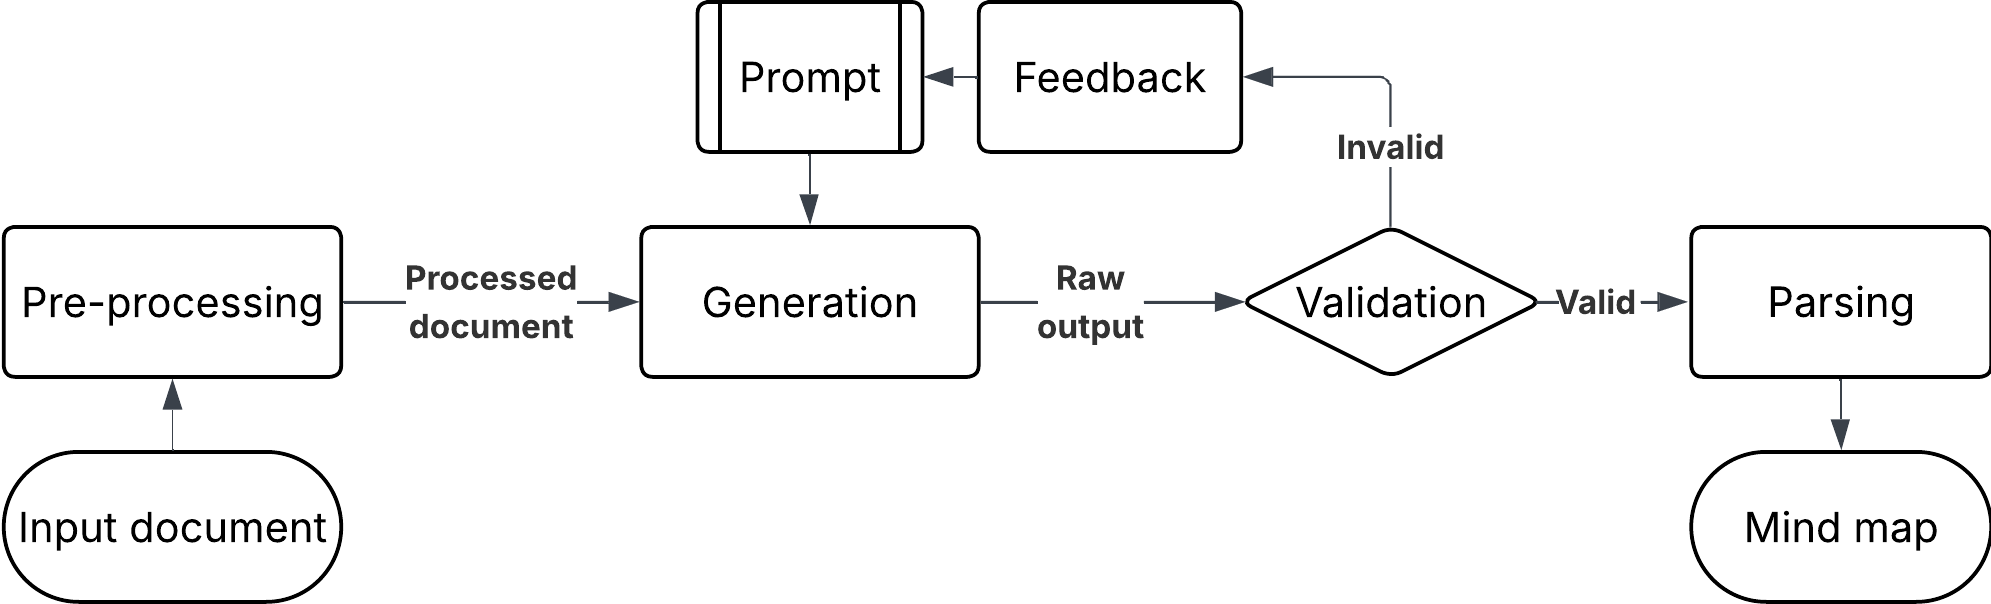
\includegraphics[width=\linewidth]{pipeline.png}
    \caption{The proposed mind map generation pipeline}
    \label{fig:pipeline}
\end{figure}



\section{Dataset}
\label{sec:dataset}
The proposed method will be tested on the mind map dataset proposed in \cite{wei2019revealing}~--- specifically, the test split, as the proposed model doesn't require training. The dataset was built by randomly selecting 135 news articles from the CNN news corpus \cite{hermann2015teaching}. For every article, one annotator wrote the mind-map and the other reviewed the output. 

The size of the dataset is about 60,000 words. The average length of the news articles, according to \cite{wei2019revealing} is about 956 words. The dataset is split into development and testing subsets, with 15 and 120 articles respectively. The development set is used for few-shot prompting and development tests, and the testing set is used to evaluate the models. The dataset is available for research purposes\footnote{https://github.com/hmt2014/MindMap}.



\section{Experiments}
\subsection{Metrics}
\label{sec:metrics}
Following other works on the task at hand, the ROUGE-based similarity metric proposed by \cite{wei2019revealing} will be used. This metric is calculated by first using a greedy strategy to find the matching parts of two mind-maps to truncate the generated tree to the size of the reference one. Then, for each pair of parent-child nodes in the reference mind map, the algorithm finds the most similar pair in the generated mind map, measures their similarity using ROUGE \cite{lin2004rouge} and removes the selected pair. The final score is calculated as the average similarity score for all matched pairs. Mathematically speaking, the metric is defined as follows:
$$
\text{Sim}(M, M') = \max\limits_{P\subset E\times E'} \sum\limits_{(e, e')\in P}\left(\text{ROUGE}(e_0, e'_0) + \text{ROUGE}(e_1, e_1')\right),
$$
where $M$, $M'$ are the compared mind maps, $E$ and $E'$ are the sets of their edges respectively and ROUGE can denote ROUGE-1, ROUGE-2 and ROUGE-L similarity scores or their mean. This similarity metric returns a score ranging from zero to one, which is convenient for averaging across mind maps of different sizes. Higher scores indicate higher similarity with reference maps, which is better.

\subsection{Experiment Setup}
For the experiment, two different LLMs are used: Qwen2.5-3B-Instruct and Qwen3-4B-Instruct. These models were selected due to their compact size, instruction-following tuning and free access to their weights, which makes them perfect for future experiment reproduction and validation. The models were both inferenced on an 8 GB NVIDIA GeForce RTX 3070 laptop GPU. Qwen3-4B-Instruct was inferenced in 4-bit quantization to avoid weight offloading and increase inference speed. The generation temperature was set to 0 to ensure compliance with the output formatting rules.

\subsection{Baselines}
The performance of the proposed method is compared with the following methods:
\begin{enumerate}
    \item \textbf{Random} selection of the graph from the document;
    \item \textbf{MRDMF}~--- the model proposed in \cite{wei2019revealing};
    \item \textbf{EMGN}~--- the method described in \cite{hu2021efficient};
    \item \textbf{CMGN}~--- the method introduced in \cite{zhang2024coreference}, the current state of the art in automatic sentence-based mind map generation.
\end{enumerate}
The evaluation results for these methods are taken from the most recent paper of all the papers listed above~--- the paper  \cite{zhang2024coreference}.

\section{Results}

\begin{table}[]
    \centering
    \begin{tabular}{c|c|cccc}
        \toprule
        \multicolumn{2}{c}{\textbf{Models}} \vline & \textbf{R-1} & \textbf{R-2} & \textbf{R-L} & \textbf{Avg} \\
        \midrule
        \multirow{4}{*}{Baselines} & Random & 32.71 & 23.51 & 30.08 & 28.77 \\
        & MRDMF & 38.19 & 29.51 & 35.72 & 34.47 \\
        & EMGN & 46.14 & 38.21 & 43.84 & 42.73 \\
        & CMGN & 47.73 & 39.75 & 45.33 & 44.27 \\
        \midrule
        \multirow{4}{*}{Qwen2.5-3B-Instruct} & 0-shot & 38.22 & 32.26 & 36.59 & 35.11 \\
        & 1-shot & 44.03 & 38.37 & 43.12 & 41.58 \\
        & 2-shot & 39.75 & 33.31 & 38.35 & 37.05 \\
        & 3-shot & 40.75 & 34.07 & 39.31 & 38.29 \\
        \midrule
        \multirow{4}{*}{Qwen3-4B-Instruct} & 0-shot & 46.51 & 40.48 & 45.18 & 44.06 \\
        & 1-shot & \textbf{49.20} & \textbf{43.18} & \textbf{48.17} & \textbf{46.83} \\
        & 2-shot & 46.55 & 40.61 & 45.53 & 43.96 \\
        & 3-shot & 46.76 & 40.92 & 45.64 & 44.24 \\
        \bottomrule
    \end{tabular}
    \caption{Evaluation results for different models.}
    \label{tab:evaluation}
\end{table}

The evaluation results are presented in Table~\ref{tab:evaluation}. Here, R-1, R-2, R-L and Avg stand for the map similarity metric's variants based on ROUGE-1, -2, -L and their mean respectively (see section~\ref{sec:metrics}). The highest scores on the test set in terms of all metrics have been achieved by Qwen3-4B-Instruct with a 1-shot prompting strategy, with its scores successfully surpassing CMGN, the previous state of the art. This indicates that the LLM-generated mind maps have achieved higher similarity with human references than previous methods. The 1-shot strategy proved to be optimal in the case of both tested LLMs. This can be due to the fact that, while few-shot guidance helps the model understand what it needs to generate, many examples can overload the context of a smaller LLM, negatively impacting performance.

A sample output of the model compared to a reference map is presented in Table~\ref{tab:example}. It represents a tendency in the LLMs outputs: they tend to be more lengthy and inclusive than references. This is not necessarily disadvantageous, given that the hierarchical structure allows for a more consice and general overview of the information in the mind map if necessary. The hierarchical relations between the nodes in the map are fairly logical, which supports the validity of the model's outputs. 

\begin{table}[]
    \centering
    \begin{tabular}{|l|l|}
\hline
\textbf{Generated} & \textbf{Reference} \\
\hline
Los Angeles (CNN) -- Comic actor... & Los Angeles (CNN) -- Comic actor... \\
1. Good Samaritans helped the... & 1. Good Samaritans helped the... \\
1.1. Arlene Van Dyke posted video... & 2. Arlene Van Dyke posted video... \\
2. Fast Facts: Dick Van Dyke... & 3. Publicist Bob Palmer said Van... \\
2.1. Van Dyke won three Emmy... &  \\
2.2 He won another Emmy for... & \\
\hline
    \end{tabular}
    \caption{Example of a generated and reference mind map.}
    \label{tab:example}
\end{table}

\begin{table}[]
    \centering
    \begin{tabular}{c|c}
    \toprule
        \textbf{Model} & \textbf{Time per map (s)} \\
    \midrule
        MRDMF & 3.89 \\
        EMGN & 0.09 \\
        CMGN & \textbf{0.03} \\
        Qwen2.5-3B-Instruct (1-shot) & 33.33 \\ 
        Qwen3-4B-Instruct (1-shot) & 85.79 \\ 
    \bottomrule    
    \end{tabular}
    \caption{Inference times for different models}
    \label{tab:time}
\end{table}

An important thing to consider is inference speed. The average inference times for different methods are presented in Table~\ref{tab:time}. We can see that while LLMs can achieve noticeably higher scores than graph-based methods, the inference times for LLM-based methods are orders of magnitude higher. It should be noted though that inference speeds for LLMs vary significantly across different models and hardware, with larger, more sophisticated LLMs providing much faster text generation than small LLMs used in this project.

% In this section, you need to list and describe the achieved results. It is crucial to have the results of the experiments for the other approaches. This is needed to be able to compare your results with some competitors. Most preferably, you should provide some references with results on the same problem.

% Almost inevitably the results are presented as a table, but it is also possible to have a graph, i.e. a figure.

% You need also to provide an interpretation of the presented results, to describe some features. E.g. your approach shows higher results on the short texts or by one metric instead of another.

% Also in this section, you could provide some results for your model inference. The samples could be found in Tab.~\ref{tab:output}.



\section{Conclusion}
This study investigated the use of LLMs for automatic sentence-based mind map generation. A novel mind map generation pipeline was created, implementing generation using lightweight LLMs. Experimental evaluation showed that the task can be solved with high quality using even lightweight modern LLMs. The experiment proved that such models can, given the right prompts and output examples, achieve state-of-the-art scores compared to previous methods based on graph models. This proves that LLMs have become a versatile tool for generating different representations of text, and with proper guidance they can be used to efficiently organize knowledge in user-friendly ways, helping achieve better retention and understanding of complex information.

\bibliographystyle{apalike}
\bibliography{lit}

\newpage

\appendix

\section*{Appendix}
\label{sec:appendix}

\begin{table}[!tbh]
    \centering
    \begin{tabular}{|l|}
\hline
You generate sentence-based mind maps for news articles. \\
\\
Task:\\
Given a numbered article, choose important sentence IDs and \\
organize them into a hierarchical numbered list.\\
\\
A good mind map:\\
- has one root sentence that represents the main topic;\\
- has several main branches for different topics or sections;\\
- places details under the branch they explain;\\
- uses parent -> child relations where the child gives more \\
specific information about the parent.\\
\\
Output format:\\
- Output only a hierarchical numbered list.\\
- The first line must be the root node.\\
- Every line must contain exactly one source sentence ID in square brackets.\\
- Copy the sentence text after the ID.\\
- Do not output JSON.\\
- Do not output explanations or markdown bullets.\\
\\
Required format:\\
{[0]} Root sentence text\\
1. [3] First major branch sentence text\\
1.1. [4] Detail sentence text\\
1.2. [5] Another detail sentence text\\
2. [10] Second major branch sentence text\\
2.1. [11] Detail sentence text\\
\\
Meaning:\\
- The first line is the root.\\
- Lines like "1.", "2.", "3." are children of the root.\\
- Lines like "1.1.", "1.2." are children of "1.".\\
- Lines like "1.2.1." are children of "1.2.".\\
\\
Rules:\\
- Use only sentence IDs from the article.\\
- Each selected sentence ID should appear only once.\\
- The hierarchy must be connected.\\
- Do not include sentence IDs that are not in the article.\\
- Do not invent or rewrite sentences.\\
\hline
    \end{tabular}
    \caption{System prompt for mind map generation.}
    \label{tab:system_prompt}
\end{table}

\begin{table}[!tbh]
    \centering
    \begin{tabular}{|l|}
\hline
Article:\\
\{numbered\_doc\}\\
\\
Generate the hierarchical mind-map list for this article.\\
\hline
    \end{tabular}
    \caption{User prompt for mind map generation.}
    \label{tab:user_prompt}
\end{table}

\begin{table}[!tbh]
    \centering
    \begin{tabular}{|l|}
\hline
The previous hierarchical list was invalid.\\
\\
Fix these issues:\\
\{feedback\}\\
\\
Return a new hierarchical numbered list only.\\
\\
Use this format:\\
{[0]} Root sentence text\\
1. [3] Child sentence text\\
1.1. [4] Detail sentence text\\
\\
Do not output JSON, explanations, or markdown bullets.\\
\hline
    \end{tabular}
    \caption{User prompt for mind map generation.}
    \label{tab:user_prompt}
\end{table}



\end{document}
